%%% The main file. It contains definitions of basic parameters and includes all other parts.

%% Settings for single-side (simplex) printing
% Margins: left 40mm, right 25mm, top and bottom 25mm
% (but beware, LaTeX adds 1in implicitly)
\documentclass[12pt,a4paper]{report}
\setlength\textwidth{145mm}
\setlength\textheight{247mm}
\setlength\oddsidemargin{15mm}
\setlength\evensidemargin{15mm}
\setlength\topmargin{0mm}
\setlength\headsep{0mm}
\setlength\headheight{0mm}
% \openright makes the following text appear on a right-hand page
\let\openright=\clearpage

%% Settings for two-sided (duplex) printing
% \documentclass[12pt,a4paper,twoside,openright]{report}
% \setlength\textwidth{145mm}
% \setlength\textheight{247mm}
% \setlength\oddsidemargin{14.2mm}
% \setlength\evensidemargin{0mm}
% \setlength\topmargin{0mm}
% \setlength\headsep{0mm}
% \setlength\headheight{0mm}
% \let\openright=\cleardoublepage

%% Generate PDF/A-2u
\usepackage[a-2u]{pdfx}

%% Character encoding: usually latin2, cp1250 or utf8:
\usepackage[utf8]{inputenc}

%% Prefer Latin Modern fonts
\usepackage{lmodern}

%% Further useful packages (included in most LaTeX distributions)
\usepackage{amsmath}        % extensions for typesetting of math
\usepackage{amsfonts}       % math fonts
\usepackage{amsthm}         % theorems, definitions, etc.
\usepackage{bbding}         % various symbols (squares, asterisks, scissors, ...)
\usepackage{bm}             % boldface symbols (\bm)
\usepackage{graphicx}       % embedding of pictures
\usepackage{fancyvrb}       % improved verbatim environment
\usepackage{natbib}         % citation style AUTHOR (YEAR), or AUTHOR [NUMBER]
\usepackage[nottoc]{tocbibind} % makes sure that bibliography and the lists
			    % of figures/tables are included in the table
			    % of contents
\usepackage{dcolumn}        % improved alignment of table columns
\usepackage{booktabs}       % improved horizontal lines in tables
\usepackage{paralist}       % improved enumerate and itemize
\usepackage[usenames, dvipsnames]{xcolor}  % typesetting in color

\usepackage[colorinlistoftodos,prependcaption,textsize=tiny]{todonotes}

%%% Basic information on the thesis

% Thesis title in English (exactly as in the formal assignment)
\def\ThesisTitle{Taxi service back-end}

% Author of the thesis
\def\ThesisAuthor{Lukáš Březina}

% Year when the thesis is submitted
\def\YearSubmitted{2018}

% Name of the department or institute, where the work was officially assigned
% (according to the Organizational Structure of MFF UK in English,
% or a full name of a department outside MFF)
\def\Department{Department of Distributed and Dependable Systems}

% Is it a department (katedra), or an institute (ústav)?
\def\DeptType{Department}

% Thesis supervisor: name, surname and titles
\def\Supervisor{doc. RNDr. Tomáš Bureš, Ph.D.}

% Supervisor's department (again according to Organizational structure of MFF)
\def\SupervisorsDepartment{Department of Distributed and Dependable Systems}

% Study programme and specialization
\def\StudyProgramme{Softwarové a datové inženýrství}
\def\StudyBranch{Databáze a web}

% An optional dedication: you can thank whomever you wish (your supervisor,
% consultant, a person who lent the software, etc.)
\def\Dedication{%
Dedication.
}

% Abstract (recommended length around 80-200 words; this is not a copy of your thesis assignment!)
\def\Abstract{%
	Nowadays services like Uber start to surpass taxi companies in comfort of transport. The goal of this thesis is to create a back-end part of the application, which will increase the taxi services efficiency and give the users new and more comfortable ways to use them. 
}

% 3 to 5 keywords (recommended), each enclosed in curly braces
\def\Keywords{%
{Taxi} {Ruby on Rails}
}

%% The hyperref package for clickable links in PDF and also for storing
%% metadata to PDF (including the table of contents).
%% Most settings are pre-set by the pdfx package.
\hypersetup{unicode}
\hypersetup{breaklinks=true}

% Definitions of macros (see description inside)
%%% This file contains definitions of various useful macros and environments %%%
%%% Please add more macros here instead of cluttering other files with them. %%%

%%% Minor tweaks of style

% These macros employ a little dirty trick to convince LaTeX to typeset
% chapter headings sanely, without lots of empty space above them.
% Feel free to ignore.
\makeatletter
\def\@makechapterhead#1{
  {\parindent \z@ \raggedright \normalfont
   \Huge\bfseries \thechapter. #1
   \par\nobreak
   \vskip 20\p@
}}
\def\@makeschapterhead#1{
  {\parindent \z@ \raggedright \normalfont
   \Huge\bfseries #1
   \par\nobreak
   \vskip 20\p@
}}
\makeatother

% This macro defines a chapter, which is not numbered, but is included
% in the table of contents.
\def\chapwithtoc#1{
\chapter*{#1}
\addcontentsline{toc}{chapter}{#1}
}

% Draw black "slugs" whenever a line overflows, so that we can spot it easily.
\overfullrule=1mm

%%% Macros for definitions, theorems, claims, examples, ... (requires amsthm package)

\theoremstyle{plain}
\newtheorem{thm}{Theorem}
\newtheorem{lemma}[thm]{Lemma}
\newtheorem{claim}[thm]{Claim}

\theoremstyle{plain}
\newtheorem{defn}{Definition}

\theoremstyle{remark}
\newtheorem*{cor}{Corollary}
\newtheorem*{rem}{Remark}
\newtheorem*{example}{Example}

%%% An environment for proofs

%%% FIXME %%% \newenvironment{proof}{
%%% FIXME %%%   \par\medskip\noindent
%%% FIXME %%%   \textit{Proof}.
%%% FIXME %%% }{
%%% FIXME %%% \newline
%%% FIXME %%% \rightline{$\square$}  % or \SquareCastShadowBottomRight from bbding package
%%% FIXME %%% }

%%% An environment for typesetting of program code and input/output
%%% of programs. (Requires the fancyvrb package -- fancy verbatim.)

\DefineVerbatimEnvironment{code}{Verbatim}{fontsize=\small, frame=single}

%%% The field of all real and natural numbers
\newcommand{\R}{\mathbb{R}}
\newcommand{\N}{\mathbb{N}}

%%% Useful operators for statistics and probability
\DeclareMathOperator{\pr}{\textsf{P}}
\DeclareMathOperator{\E}{\textsf{E}\,}
\DeclareMathOperator{\var}{\textrm{var}}
\DeclareMathOperator{\sd}{\textrm{sd}}

%%% Transposition of a vector/matrix
\newcommand{\T}[1]{#1^\top}

%%% Various math goodies
\newcommand{\goto}{\rightarrow}
\newcommand{\gotop}{\stackrel{P}{\longrightarrow}}
\newcommand{\maon}[1]{o(n^{#1})}
\newcommand{\abs}[1]{\left|{#1}\right|}
\newcommand{\dint}{\int_0^\tau\!\!\int_0^\tau}
\newcommand{\isqr}[1]{\frac{1}{\sqrt{#1}}}

%%% Various table goodies
\newcommand{\pulrad}[1]{\raisebox{1.5ex}[0pt]{#1}}
\newcommand{\mc}[1]{\multicolumn{1}{c}{#1}}


% Title page and various mandatory informational pages
\begin{document}
%%% Title page of the thesis and other mandatory pages

%%% Title page of the thesis

\pagestyle{empty}
\hypersetup{pageanchor=false}
\begin{center}

\centerline{\mbox{
\includegraphics[width=166mm]{../img/logo-en.pdf}}}

\vspace{-8mm}
\vfill

{\bf\Large BACHELOR THESIS}

\vfill

{\LARGE\ThesisAuthor}

\vspace{15mm}

{\LARGE\bfseries\ThesisTitle}

\vfill

\Department

\vfill

\begin{tabular}{rl}

Supervisor of the bachelor thesis: & \Supervisor \\
\noalign{\vspace{2mm}}
Study programme: & \StudyProgramme \\
\noalign{\vspace{2mm}}
Study branch: & \StudyBranch \\
\end{tabular}

\vfill

% Zde doplňte rok
Prague \YearSubmitted

\end{center}

\newpage

%%% Here should be a bound sheet included -- a signed copy of the "bachelor
%%% thesis assignment". This assignment is NOT a part of the electronic
%%% version of the thesis. DO NOT SCAN.

%%% A page with a solemn declaration to the bachelor thesis

\openright
\hypersetup{pageanchor=true}
\pagestyle{plain}
\pagenumbering{roman}
\vglue 0pt plus 1fill

\noindent
I declare that I carried out this bachelor thesis independently, and only with the cited
sources, literature and other professional sources.

\medskip\noindent
I understand that my work relates to the rights and obligations under the Act No.~121/2000 Sb.,
the Copyright Act, as amended, in particular the fact that the Charles
University has the right to conclude a license agreement on the use of this
work as a school work pursuant to Section 60 subsection 1 of the Copyright Act.

\vspace{10mm}

\hbox{\hbox to 0.5\hsize{%
In ........ date ............	% FIXME!
\hss}\hbox to 0.5\hsize{%
signature of the author
\hss}}

\vspace{20mm}
\newpage

%%% Dedication

\openright

\noindent
\Dedication

\newpage

%%% Mandatory information page of the thesis

\openright

\vbox to 0.5\vsize{
\setlength\parindent{0mm}
\setlength\parskip{5mm}

Title:
\ThesisTitle

Author:
\ThesisAuthor

\DeptType:
\Department

Supervisor:
\Supervisor, \SupervisorsDepartment

Abstract:
\Abstract

Keywords:
\Keywords

\vss}

\newpage

\openright
\pagestyle{plain}
\pagenumbering{arabic}
\setcounter{page}{1}


%%% A page with automatically generated table of contents of the bachelor thesis

\tableofcontents

%%% Each chapter is kept in a separate file
\chapter{Introduction}


We have implemented first version of application in Individual Software Project which is up and running since July 2017. When I refer to the first version of application I mean this.
\section{Goals}
This theses has three main goals
\begin{itemize}
	\item Create application covering order management with respect to existing taxi company processes
	\item Provide API for front-end(s) which is
	\begin{itemize}
		\item secure,
		\item well documented,
		\item easy to use,
		\item general enough for later extension to other front-end services
	\end{itemize}
	\item Put together stack of tools which allows:
	\begin{itemize}
		\item easy deployment with minimal down time,
		\item quick installation,
		\item operation system independence,
		\item developer-friendly errors \& system monitoring,
		\item back-ups
	\end{itemize}
\end{itemize}

\section{Outline}
\chapter{Requirements}
In the first part of the chapter we focus on the analysis of creating wholesome solution for taxi company and related business requirements. In the second part we specify requirements from the technical point of view - whether back-end or cooperating front-end. In the end we specify individual parts of back-end application and what they should fullfill.
\section{Business requirements  \todo{JUST DRAFT! write in sentences, structure it}} 
\begin{itemize}
	\item Handle order system - staff fluctuation is high, train employees is expensive - especially dispatchers, which must have good estimate
	\item Allow customers to order directly via their phone apps or other sources - saving costs of dispatching. Because it is very easy to order via phone call make it as easy as possible
	\item Customers must have overview how much their order will approximetly cost and must be able to select their driver. Also they must have approximate estimate when their taxi will come.
	\item Customers should be informed about their ordered driver status - where he is and when them will come
	\item better customer service - remember name, favorite location, other things
	\item security - strong competition, already few cases of hacking and data stealing
	\item some of the things written tailored for our local taxi company but should be easily rewritten and reused for some other company with differnet requirements and priorities
	\item predicted data size for the project for now: 10 drivers - 7 online, 7 cars, 10 dispatchers - 2 online, 6000 customers, 800 orders per week
	\item authorization
	\item two main types of orders - scheduled on time and normal. Our high priority is to be there for scheduled precisely on time.
	\item handling frauds
\end{itemize}
\section{Technical requirements}
\begin{itemize}
	\item Separate back-end and frontend - allows more customization on frontend which can and will change more frequently totally independently on backend. On frontend - where are apps and PWAs and orders through FB messenger for example.
	\item HTTPS
	\item Frontend-developer friendly instalation and independency
	\item Able to install easily on new server with possibility to scale - at least preparation
	\item Errors logging and alerting
\end{itemize}

\chapter{Analysis}
In this chapter we would like to explain the thinking process before and during the implementation of the back-end application. We are going through individual parts from the back-end application requirements, explaining problems associated with them and revealing what possibilities we had to solve them and how we decided in the end.

\section{General problems}
\subsection{Authentication}
In our application we had to deal with authentication for customers and employees. There are many ways how users can be authenticated in API. We ended up with token authentication - in each request clients must set the Authorization header with the token. Client can get the token in exchange for correct credentials.

Another part of the authentication we consider in the analysis is at least the basic security during the manipulation with auth data and flawless verifying token sending.

\subsubsection{Token authentication details}

We decided to implement it on our own, using only Rails helpers for generating and verifying secure tokens. As you can see in \ref{auth-token-scheme}, token is generated during the login action and then returned in body of the response. All the following requests must have this token in it's header to be authenticated.

\begin{figure}[h]\centering
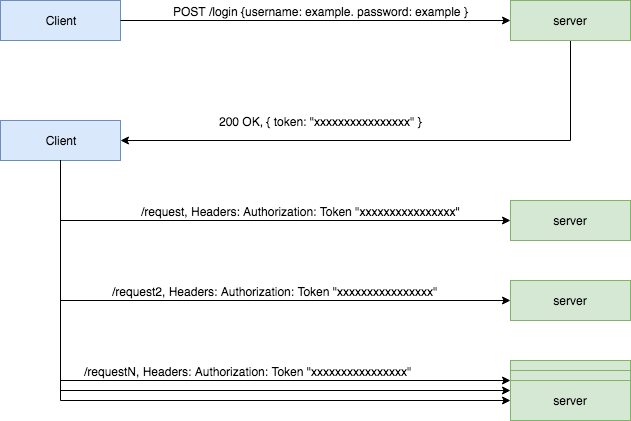
\includegraphics[width=\textwidth]{auth/Auth.png} 
\caption{Auth token scheme}\label{auth-token-scheme}
\end{figure}

Our application store just one token per user. That implies the user can be logged in from one device at time only. Having more valid token for users would let into several problems with invalidating them in case of log out and also this approach has one advantage. If someone reveals user credentials and log in with them - user will know that in the moment it tries to use the app, because all it's requests would be unauthenticated.

In Ruby on Rails there exists very good gem for authentication - \textit{devise\_token\_auth} \footnote{\url{https://github.com/lynndylanhurley/devise\_token\_auth}} which we half-implemented at first. However we decided to not use it in the end. Main reason for not using it was - at the time of writing the authentication part - very unstable and badly documented front-end library part. More details about problems we came across during the analysis/implementation in the next paragraph.

First reason for not using the gem was, that it uses email as main default authentication field. For customers we wanted to use the telephone number as the main identifier - including the SMS confirmation and password recovery (explained later), which would led us to rewrite the most of the gem's controllers and models anyway and as bonus we would have to integrate it with the existing parts of gem.

Second reason was the complexity of the whole authentication process. This gem would bring to our project more secure but also much more complex way of authenticating. Once client gets the token from the login endpoint, the token is generated and returned with each following request. Using this approach we have to solve the batch request problem. Imagine that client sends for example three requests at once to the server. Of course all the three requests must have same authentication token - because client doesn't have the new token until the response comes. Thus server must accept all those three requests as authenticated, but also they must agree with the front-end which response has the correct new auth token - responses don't have to come in order in which they were sent. This complicated process was implemented in the back-end gem and couldn't be changed. The front-end library was supposed to implement that, but after the three weeks of trying and founding several bugs in the library - even without successful login they gave up using it.

In conclusion if we had wanted to use the gem on backend we would have to understand the whole gem auth process in detail and specify it for the front-end. Front-end would then have to write the whole complicated solution on their own. 

We came to conclusion that the complexity, that would bring this library to our application is not worth the better security and stability we would gain from this. Using HTTPS on both server and client makes the token theft little bit harder - so lack of this generation process with each request is not a big deal. Also the only really sensitive accounts for identity theft are the employees one's and we are in personal contact with them, so we would know about misuse or potential hack and we could provide the safer solution later.

\subsubsection{Basic security}
As we mentioned in last paragraphs, our token solution is not perfect from the security perspective. Besides the token (which could be easily rewritten more securely in the future ) we tried not to take the security of our application lightly.

First of all, we don't store passwords in plaintext. We use Rails integrated feature \textit{has\_secure\_password}\footnote{\url{https://api.rubyonrails.org/classes/ActiveModel/SecurePassword/ClassMethods.html}}, which uses BCrypt hash function.

Thanks to the Ruby on Rails framework we also excerpt passwords from the logs and we are not vulnerable to SQL Injection\footnote{\url{https://en.wikipedia.org/wiki/SQL\_injection}}.

\subsubsection{Sending verifying tokens}
We must send tokens via emails and SMS during the whole authentication process. Because these are actions that are not instant (API request, SMTP request) and because in Rails we can easily create asynchronous workers, we decided to have these functions handled as Sidekiq workers. In exchange for some time spent on configuration we have instant response without blocking webserver threads during account creation/recovery and have ability to automatically resend the message in case of the third party or network failure.

\subsection{Authorization}
Almost every endpoint has it's own rules of who and in what circumstances can do such action. There are two main groups of users - employees and customers. Employees are then divided into three groups - administrators, drivers and dispatchers. There are just two types of customers - registered and unregistered. Each visitor is one of these types.

In each request we have to solve specific condition whether current user is able to do this action or not. Having the all these conditions directly in controllers would make the controllers difficult to read. Also these conditions could change in the future and have changed during the development several times. This led us to have the authorization conditions separated in the different part of the application.

We want to avoid reinventing the wheel so we have chosen to use for such purpose \textit{Pundit} \footnote{\url{https://github.com/varvet/pundit}} gem. 

Another option we looked into was \textit{Cancancan} \footnote{\url{https://github.com/CanCanCommunity/cancancan}} gem. They both have long maintenance history, are actively developed in the time of writing and satisfies all of our conditions for the authorization. Cancancan is better suited for applications with complicated views, because it provides more helpers for checking authorization in them. Also its architecture is more general thus it is better optimized for more complicated permission management. That results in slightly more complex permission definitions. On the other side pundit is more light-weight solution with very simple architecture and permissions definition files. Because our permissions are not complicated very much and we wanted to have them written as simply as possible, this was the main reason why we chose Pundit over Cancancan.

 \subsection{Pagination}
 paginating lists - why, where
\subsection{Request parameters security}
Permiting

\subsection{Rendering views}
\subsection{Localization}
- more languages - errors
 - we translate on our side, frontend on its => bad pattern
\subsection{Images}
	- too difficult for front-end to implement and handle api multipart requests
	- limitation only one image for entity => but enough for us
	- employee and vehicle images


\section{Customers}
Use email as main distinguishing field is kind of standard in web authentication. We came to the conclusion that we should use as our identifier telephone number. Despite the standard and the the consequence of this decision - lack of any easy to use library for authentication in Rails. Reasons which led us to this decision:
\begin{itemize}
	\item During the order process we must be able to contact customer immediately in case of emergency, so we need the customer's phone anyway.
	\item Customers are going to register mostly from their phones. That phone can receive SMS for sure - not everyone has direct access to his mail from phone. 
\end{itemize}
\subsection{Create and confirm}
Besides the authentication and params problems \todo{give links} described in general problems section we also have to to deal with the telephone verification.

We decided to use verification via SMS code.

 Registered telephone number must be verified.  Before the customers can do so, they must go through telephone number confirmation process as follows: Customers receive SMS with registration token. This token is valid for 5 minutes and customer can ask for resend.  Resend will invalidate last token, generate new and send it. Confirm is made with provided token and telephone number.
 
 Based on requirements we decided to split these functions into three API endpoints - \textit{create}, \textit{confirm} and \textit{resend\_confirmation}.
 
 \subsection{Password recovery}
 Whole password recovery procedure is similar to the create account one.
 Based on specification we split the password recovery feature into two API endpoints - \textit{password\_recovery} and \textit{reset\_password\_by\_token}. 
 
 Calling first endpoint - password recovery - sends in exchange for the telephone number SMS to that telephone number with password recovery token. Then the customer can send request with this token, his telephone number and a new password - which if all the conditions are satisfied - will be set. 
 
 The token consists of 4 numbers and is valid for 5 minutes. This parameters we just picked as similar to the others services on the internet and of course we must be able to change them later if we discover that it's not good.
 
 During the analysis we have noticed, that the first endpoint must except the bad request format always return success status. Especially, we can not let the client know whether the account with such telephone number was not found and neither that the SMS was not sent successfully. If we would return error code in such situation, someone could potentially get the telephone numbers for all of our customers.
 
 Also we are aware that the SMS may not be the most secure way of verifying users\footnote{\url{https://www.cnet.com/how-to/why-you-are-at-risk-if-you-use-sms-for-two-step-verification/}} but we think that at our scale, potential losses for stolen customer's account wouldn't be crucial - there is no credit system or something valuable on the account. The worst case is that the attacker orders a taxi on victims name and thus that order will be fraud - which happens few times a week now anyway.
 
 \subsection{Favourite places}
 We decided to have an endpoint with four parameters, which will return the list of N recommended places ordered from the most to the least appropriate.
 
 First is parameter is the maximum number of places we would like to receive, second is customer id for whom we want to have recommendations for, third is the location and the last - 'start' - parameter  says one of the following:
 \begin{itemize}
 	\item true = we want recommendations for pick-up places and the provided location are customer's current coordinates
 	\item false = we want recommendations for drop-off locations and the provided location are pick-up coordinates
 \end{itemize}
 
 Our first problem to solve was how to handle locations from the request. We suppose that the location which goes to our API is directly from the customer's telephone sensors, thus there's nothing like Example's restaurant official coordinates, which would client sent to us whenever he wants taxi from that restaurant. On the other hand, we would like to group all these locations near the Example restaurant into one place, so we can recommend it just once and there was enough space for other interesting places. We thought about using some kind of modified clustering algorithm but we ended up with conclusion that this would be in our case overkill. We came to conclusion that for our use case is enough to have defined distance constant and all the places around this place within the constant distance are considered as one place. We set this constant to 50 meters, because it seems like good compromise between inaccurate low-end phones GPS precision and the distance between two different places. Of course that we must be able to change this constant in the future if we discover, that it is too small or big.
 
 Second problem was how to filter and return the list of places fast. For each user we have index of visited places with information on which we base our recommending algorithm. In this index we have following information about each place:
 \begin{itemize}
 	\item coordinates
 	\item list of items containing for each place occurrence in orders:
 	\begin{itemize}
 		\item decimal number from 0 to 1 which says, how long ago was order with this place placed. 1 has user's last order and 0 has user's furthermost order .
 		\item time-stamp when was the order created
 		\item start = whether was the place in the order used as a start or finish
 	\end{itemize}
 	\item list of corresponding places (drop-off for pick-up and vice versa).
 \end{itemize}
For the given parameters in request, we go in index place by place and count the weight of it from the occurrences weights multiplied by constant if start/finish fits the desired direction. Index is also prepared for recommending places based on the order time (e.g. in the evening we go to pub, in the morning to work). We decided to limit the recommendation index for last 1000 orders for each user.

In our research we haven't found any ready-made solution for this problem, so we decided to come up with our own solution. Of course it could be more effective and recommendation could be done even smarter. During the development we came to this algorithm which satisfies all our specified metrics and thus we were satisfied with the application of it in the real world.


\section {Orders}
Format of times
Cost of api requets, Google API
order planning system
\begin{figure}[h]\centering
	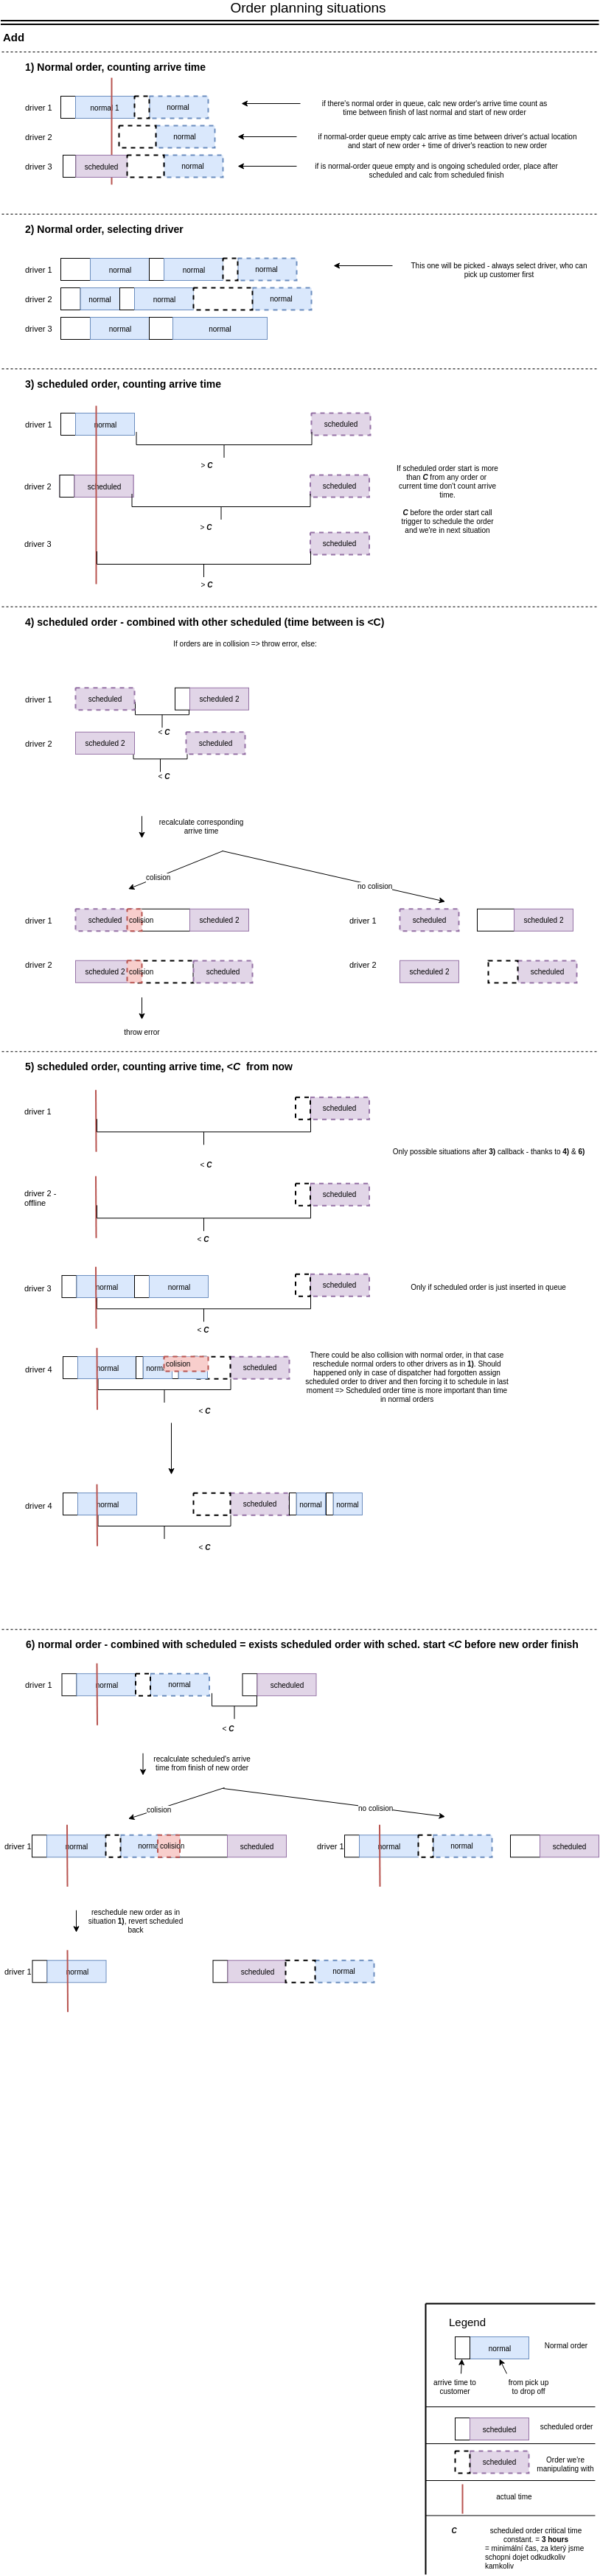
\includegraphics[scale=0.2	]{orders/order_planning.png}
	\caption{Order planning situations}\label{order-process-scheme}
\end{figure} 

\chapter{Title of the first chapter}

An~example citation: \cite{Andel07}

\section{Title of the first subchapter of the first chapter}

\section{Title of the second subchapter of the first chapter}

\chapter{Title of the second chapter}

\section{Title of the first subchapter of the second chapter}

\section{Title of the second subchapter of the second chapter}


\chapter*{Conclusion}
\addcontentsline{toc}{chapter}{Conclusion}
In our thesis we have successfully managed to create the back-end part of the application for the taxi companies. We analysed, specified and implemented the whole process of ordering and distributing the orders to the drivers. 

Besides the application itself we put together the stack of technologies which allows us to run, distribute and monitor the application.

From the technological point of view our application is ready to be used by the taxi companies in production and improve the services they provide. Unfortunately the pricing change in the API used for the route calculation made the costs per one processed order too high.

To make the project sustainable from the business point of view we would have to switch from the Google API to other route calculation API. Other possible improvements would be in the order scheduler. First of all we should separate the split the algorithm into workers so we would be able to scale the number of processed orders at once easily. Secondly after the few months of operation we could measure the estimated and final durations of the individual order parts and drastically improve the estimation system.

%%% Bibliography
%%% Bibliography (literature used as a source)
%%%
%%% We employ bibTeX to construct the bibliography. It processes
%%% citations in the text (e.g., the \cite{...} macro) and looks up
%%% relevant entries in the bibliography.bib file.
%%%
%%% The \bibliographystyle command selects, which style will be used
%%% for references from the text. The argument in curly brackets is
%%% the name of the corresponding style file (*.bst). Both styles
%%% mentioned in this template are included in LaTeX distributions.

\bibliographystyle{plainnat}    %% Author (year)
% \bibliographystyle{unsrt}     %% [number]

\renewcommand{\bibname}{Bibliography}

%%% Generate the bibliography. Beware that if you cited no works,
%%% the empty list will be omitted completely.

\bibliography{bibliography}

%%% If case you prefer to write the bibliography manually (without bibTeX),
%%% you can use the following. Please follow the ISO 690 standard and
%%% citation conventions of your field of research.

% \begin{thebibliography}{99}
%
% \bibitem{lamport94}
%   {\sc Lamport,} Leslie.
%   \emph{\LaTeX: A Document Preparation System}.
%   2nd edition.
%   Massachusetts: Addison Wesley, 1994.
%   ISBN 0-201-52983-1.
%
% \end{thebibliography}


%%% Figures used in the thesis (consider if this is needed)
\listoffigures

%%% Tables used in the thesis (consider if this is needed)
%%% In mathematical theses, it could be better to move the list of tables to the beginning of the thesis.
\listoftables

%%% Abbreviations used in the thesis, if any, including their explanation
%%% In mathematical theses, it could be better to move the list of abbreviations to the beginning of the thesis.
\chapwithtoc{List of Abbreviations}

%%% Attachments to the bachelor thesis, if any. Each attachment must be
%%% referred to at least once from the text of the thesis. Attachments
%%% are numbered.
%%%
%%% The printed version should preferably contain attachments, which can be
%%% read (additional tables and charts, supplementary text, examples of
%%% program output, etc.). The electronic version is more suited for attachments
%%% which will likely be used in an electronic form rather than read (program
%%% source code, data files, interactive charts, etc.). Electronic attachments
%%% should be uploaded to SIS and optionally also included in the thesis on a~CD/DVD.
%%% Allowed file formats are specified in provision of the rector no. 72/2017.
\appendix
\chapter{Attachments}

\section{First Attachment}

\openright
\end{document}
